\chapter{Introduction}
\label{ch:intro}

\lettrine[lines=3]{T}{he} nature of dark matter (DM) remains one of the major unsolved problems in physics. Originally inferred through its gravitational influence on galaxies and clusters, a rich body of evidence has accumulated over the last four decades firmly establishing its existence. All of the evidence, however, comes from inferring dark matter's presence solely through its gravitational effects. Many open questions remain: Does dark matter consist  of a fundamental particle? If so, what is its mass? Could there be an entire dark sector, akin to the Standard Model (SM)? How does dark matter interact with the SM? The quest to answer these questions drives a huge collective effort that draws from a rich body of theoretical and experimental work, as well as major input from computational and numerical studies. We are currently at the dawn of a data-driven era in astrophysics and cosmology---a large number of ongoing and forthcoming experiments, both in the lab and in the sky, combined with an increasingly open approach to data availability, offer great potential in elucidating the nature of dark matter. 

Dark matter plays a central role in many subfields of particle physics, astrophysics and cosmology. Understanding its nature and interactions would have far reaching consequences in those fields by providing major insights into fundamental physics beyond the Standard Model as well as elucidating the evolution of our Universe and the formation of structures within it. 

% While there exists a proliferation of ideas regarding the particle nature of dark matter, the dominant paradigm over the last three decades has been that of the Weakly Interacting Massive Particle (WIMP), which posits dark matter to consist of a particle with weak-scale interactions with the Standard Model, produced through thermal freeze-out in the early universe. This framework dovetails well, for example, with supersymmetric extensions to the Standard Model where candidates for dark matter can emerge naturally. After briefly describing alternative explanations, in this thesis I will focus exclusively on WIMP searches. I will also focus exclusively on astrophysical searches for WIMPs.

This introduction is organized as follows. In Sec.~\ref{sec:evidence}, I will summarize the large body of evidence pointing to the existence of dark matter, occasionally touching upon relevant historical developments. In Sec.~\ref{sec:particledm}, I will describe possible explanations for the particle nature of dark matter and various detection schemes, focusing on DM thermally produced in the early Universe and specifically Weakly Interacting Massive Particles (WIMPs). Section~\ref{sec:astrodm} will focus on the effort to detect and characterize WIMPs through their astrophysical signatures, in particular using gamma-ray data. I will briefly summarize the theoretical and experimental tools available to us in these searches. Finally, in Sec.~\ref{sec:summary}, I will describe the organization of the rest of this thesis. This chapter partially draws from a number of excellent review articles on the topic which the reader is referred to for further details. Refs.~\cite{Lisanti:2016jxe,Plehn:2017fdg} provide recent, comprehensive reviews of dark matter physics. Ref.~\cite{Slatyer:2017sev} reviews indirect detection, which will be the main focus of this thesis. Finally, Ref.~\cite{Bertone:2016nfn} provides a thorough overview of the history of the field.

% Wherever possible, I will touch upon the historical developments that have paved the way for our current state of understanding of dark matter and our efforts to look for it.

\section{Evidence for Dark Matter}
\label{sec:evidence}

Although the study of dark matter had its inception and development in the 20th century, the interplay between theory and observation in making the unknown knowable goes back much earlier. For example, the Aristotelian view of an immutable Universe with the Earth at its center offered a clean framework that did not call for additional celestial objects, and was the orthodox viewpoint until Renaissance astronomers conclusively refuted it with observations. Galileo was able to leverage new technological developments and make observations that arguably played the largest role in this. After pioneering the development of the telescope, he was able to understand the make-up of the Milky Way as consisting of individual stars rather than diffuse clouds, observe Saturn's rings and discover Jupiter's four largest moons. These observations are very much in the spirit of modern dark matter searches---demonstrating that the Universe can contain invisible forms of matter, and that scientific inquiry and technological developments can play a big role in revealing them to us.

% \subsection{Dynamical Evidence}

Evidence for some yet-unknown form of matter started piling up in the early 19th century. 
% Lord Kelvin introduced the idea of applying the ``theory of gases'' to the Milky Way, describing stars as gas particles acting under the influence of gravity and in the process wondering whether a large number of stars could actually be unobservable dark bodies. 
In 1922, Dutch astronomer Jacobus Kapteyn wrote down for the first time a predictive model for the distribution of matter in the Milky Way, describing the stars as particles in a virialized system~\cite{1922ApJ....55..302K} and using this model to obtain the local matter density in terms of the observed stellar mass. Kapteyn's student Jan Oort~\cite{1932BAN.....6..249O} and others~\cite{1922MNRAS..82..122J} were able to derive estimates for the local matter density, in some cases seeing excesses above the observed luminous mass. Astronomers during this time reckoned with the existence of missing matter in the Universe, in some cases explicitly using the term \emph{dark matter}~\cite{1922ApJ....55..302K} and positing that it could potentially be accounted for by the extrapolation of the stellar luminosity function down to very faint stars~\cite{1932BAN.....6..249O}.

In 1933, Swiss-American astronomer Fritz Zwicky studied redshift data for galaxy clusters collected by Hubble and Humason~\cite{1931ApJ....74...43H}, using estimates of the velocity dispersions in eight galaxies within the Coma cluster to estimate its mass through the virial theorem~\cite{1933AcHPh...6..110Z}. Zwicky obtained a theoretical prediction for the dispersion by using the number of observed galaxies, average mass of a galaxy and its extent, finding a value of $\sim$80 km\,s$^{-1}$. This was in stark conflict with the observed line-of-sight velocity dispersion of $\sim$1000 km\,s$^{-1}$. Although Zwicky's work made use of an estimate of the Hubble constant that was a factor of $\sim$8 too big compared to the current accepted value, the large discrepancy between the observed and expected values pointed to the existence of unaccounted-for matter in the Coma system. Zwicky himself concluded that ``If this would be confirmed, we would get the surprising result that dark matter is present in much greater amount than luminous matter.'' An analysis of the Virgo cluster by Sinclair Smith in 1936 again pointed to a very high mass-to-light ratio in that system. In either case, the astronomers put forward potential explanations in terms of diffuse clouds of internebular material~\cite{1937ApJ....86..217Z}.

Although this presented a conundrum, there was widespread consensus within the astronomical community that more information would be needed to understand what was going on. Historically, velocity rotation curves---the circular velocity profiles of stars in a galaxy as a function of the distance from the galactic center---did the most to convince the scientific community of the existence of large amounts of non-luminous matter in galaxies. The basic idea here is as follows. Standard Newtonian theory dictates that the circular velocity of stars is given by $v_c(r) = \sqrt{GM(r)/r}$, where $r$ is the radial distance, $M(r)$ the mass enclosed within radius $r$ and $G$ the universal gravitational constant. In the region beyond the galactic disk (which defines the observed extent of a given galaxy), we expect the enclosed mass to be constant, and consequently the circular velocity to fall as $v_c \propto r^{-1/2}$. Measurements started in the late 1930s with Babcock's observations of the rotation curve of M31 (Andromeda) out to about 20 kpc from its center~\cite{1939LicOB..19...41B}. Technological advancements over the next few decades enabled more accurate measurements. 
In the 1970s, Kent Ford, Vera Rubin and others observed in galaxies such as M31 and M33 as well as the Milky Way the approximate flattening of rotation curves at distances extending well beyond the baryonic disk~\cite{1970ApJ...159..379R,1973A&A....26..483R}. The implications of these observations for the missing mass problem were realized soon after~\cite{1974Natur.250..309E,1974ApJ...193L...1O}. Flat rotation curves indicated that the mass contained in a galaxy continues to increase as $M \propto r$ beyond the extent of the visible matter, in the form of unobserved ``dark'' matter whose density can be inferred to roughly scale as $\rho(r) \propto 1/r^2$.
% Observations by Kent Ford, Vera Rubin and others throughout the 1970s, starting with those of the nearby galaxies M31 and M33 and indeed our own Milky Way, pointed to the approximate flattening out of rotation curves at larger radii contrary to expectation with a baryonic disk alone~\cite{1970ApJ...159..379R,1973A&A....26..483R}, and implications for the missing mass problem were realized soon after~\cite{1974Natur.250..309E,1974ApJ...193L...1O}. This implied that the mass continues to increase as $M \propto r$, pointing to the existence of additional unobserved `dark' mass beyond the visible component. From this, the density of dark matter can be inferred to roughly scale as $\rho(r) \propto 1/r^2$. 
% A large number of observations on galactic and cluster scales since then have strengthened the case for the existence of halos of dark matter extending far beyond the visible extent of these objects. 
The left panel of Fig.~\ref{fig:evidence} shows the measured rotation curves for the Milky Way compiled in Ref.~\cite{2009PASJ...61..227S} compared with theoretical expectations from bulge- and disk-like components (blue and green lines, respectively) inferred from baryonic matter, as well as an additional dark matter component from a spherical, isothermal dark matter halo (red line). The rotation curve for the baryonic-only component (disk + bulge) is shown as the dashed yellow line, and the total rotation curve including the dark halo is shown as the solid yellow line. It can clearly be seen that the additional dark halo component is required to match the observed data at larger radii $r \gtrsim 15$ kpc. The descriptions of the individual components shown are provided in Ref.~\cite{2009PASJ...61..227S}.

While astrophysical observations played a significant role historically in motivating the study of dark matter, modern cosmological data provides substantial evidence supporting its existence in our Universe. $\Lambda$CDM, a phenomenological framework often referred to as the standard model of cosmology, contains dark energy ($\Lambda$) and cold dark matter (CDM) as essential ingredients. It is able to account for a plethora of cosmological observations, including the existence and structure of the cosmic microwave background (CMB) radiation, large-scale distribution of matter, accelerating expansion of the Universe and relic elemental abundances~\cite{Dodelson:1282338,Kolb:1990vq}. In particular, the CMB, which is the imprint of photons that decoupled from the baryon-photon fluid in the Universe about 370,000 years ago and have been free-streaming ever since, provides irrefutable evidence for (non-baryonic) dark matter. The primary relevant observable is the angular scale of inhomogeneities in the temperature distribution (the $TT$ angular power spectrum) of the CMB. The power spectrum largely consists of a set of peaks, each indicating an angular scale with a particularly large contribution to the temperature fluctuations. The leading physical effect behind these are acoustic oscillations in the baryon-photon fluid during photon decoupling. Early on, photons and baryons were electromagnetically coupled, and non-baryonic dark matter was responsible for generating gravitational potential wells that could pull in the baryon-photon fluid. The photon pressure acting against these wells gave rise to a tower of acoustic modes, imprinted in the CMB as characteristic peaks. While the detailed physics is somewhat nuanced\footnote{See Wayne Hu's CMB tutorials for an excellent introduction: \url{http://background.uchicago.edu/index.html}.}, the relative heights of these peaks can provide information about the energy content of our Universe, including the relative composition of baryonic and non-baryonic (dark) matter. Very heuristically, the position of the first peak provides information about the curvature of the universe (and hence how much total ``stuff'' there is in it), while the second peak tells us how much of the matter is baryonic (ordinary matter). The third peak and its relative height can shed insights into the abundance of non-baryonic dark matter. Historically, the WMAP satellite, while not able to fully resolve the third peak, was already able to conclusively say that dark matter makes up the majority of the matter budget in the Universe, finding the baryon density $\Omega_b h^2=0.02264\pm0.00050$ and cold dark matter density $\Omega_c h^2=0.1138\pm0.0045$~\cite{2013ApJS..208...19H}. Since then, \emph{Planck} has been able to precisely measure eight peaks of the $TT$ spectrum, finding $\Omega_b h^2= 0.02225\pm0.00016$ and $\Omega_c h^2=0.1198\pm0.0015$ when additionally including the CMB $E$-mode polarization auto- and cross-spectra ($EE$ and $TE$). The right panel of Fig.~\ref{fig:evidence} shows the \emph{Planck} $TT$ spectrum~\cite{Ade:2015xua} along with the best-fit theoretical predictions (solid blue line), as well as predictions for a slightly altered cosmology $\Omega_b h^2= 0.042$ and $\Omega_c h^2=0.10$ with a reduced dark matter density (dashed blue line), where striking differences from the measured spectrum can be seen.

\begin{figure}[htbp] 
\hspace{-0.9 cm} 
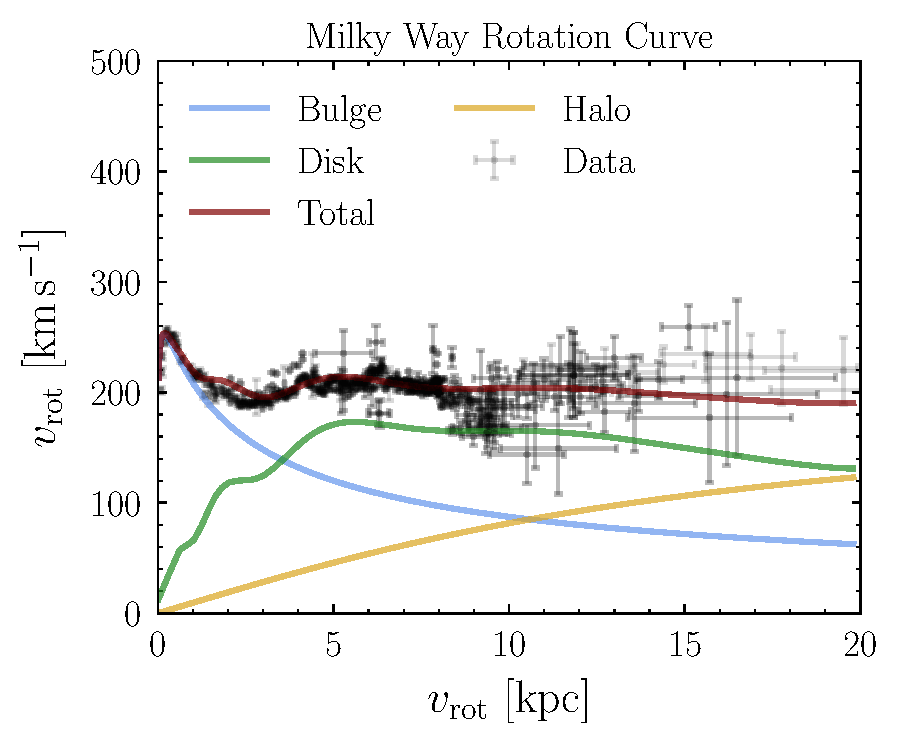
\includegraphics[width=0.5185\textwidth]{ch-intro/rotcurves.pdf}
 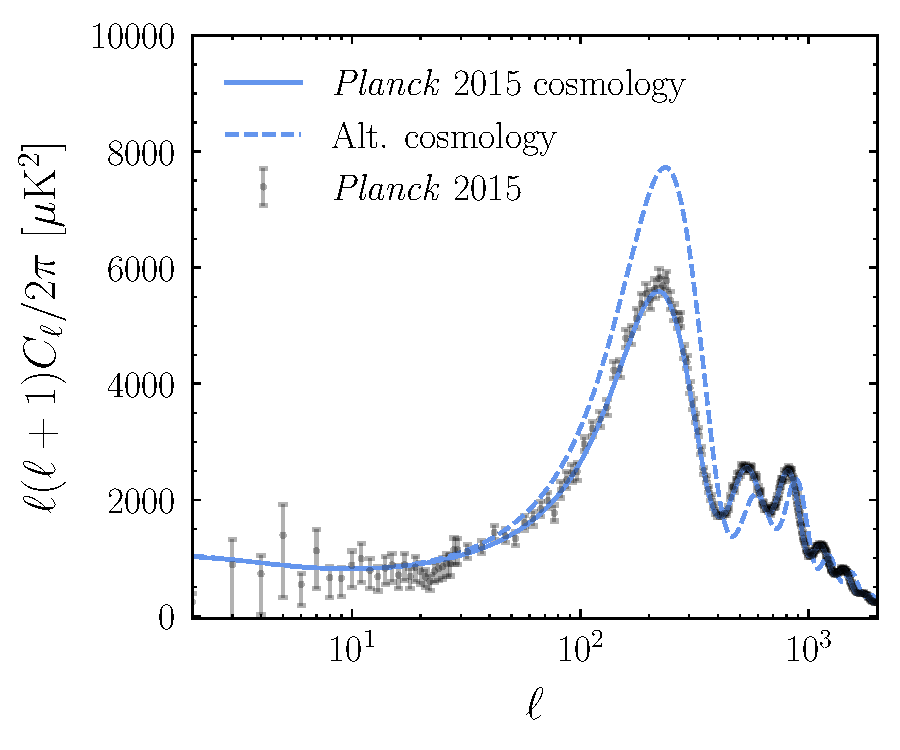
\includegraphics[width=0.528\textwidth]{ch-intro/cells.pdf}  
\caption{\textbf{(Left)} The measured rotation curves for the Milky Way compiled in Ref.~\cite{2009PASJ...61..227S}, and theoretical expectations from bulge- and disk-like components (blue and green lines, respectively) inferred from baryonic matter~\cite{2009PASJ...61..227S}, as well as an additional dark matter component from a spherical, isothermal halo (red line). The rotation curve for the baryonic-only component (disk + bulge) is shown as the dashed yellow line, and the total rotation curve including the dark halo is shown as the solid yellow line. The dark halo component is required to match the observed data at larger radii $r \gtrsim 15$ kpc. \textbf{(Right)} The \emph{Planck} $TT$ spectrum~\cite{Ade:2015xua} along with the best-fit theoretical predictions (solid blue line, computed with \texttt{CAMB}~\cite{Lewis:1999bs}), as well as predictions for a slightly altered cosmology with $\sim$10\% less non-baryonic (dark) matter (dashed blue line) where  striking differences from the observed spectrum can be seen.}  
\label{fig:evidence}
\end{figure}

The above classes of observational evidence or the existence of DM are by no means exhaustive---many other observations over a large range of scales support the existence of dark matter, including observations of the distribution of galaxies on large scales~\cite{Alam:2016hwk}, weak~\cite{Abbott:2017wau} and strong lensing~\cite{2010MNRAS.408.1969V,2012Natur.481..341V} of background galaxies by foreground structure, and observations of merging clusters~\cite{Clowe:2006eq}.

\section{(Particle) Nature of Dark Matter}
\label{sec:particledm}

Although there exists a great deal of evidence for the existence of dark matter, its nature largely remains a mystery. These days, it is often implicitly assumed that when people are talking about detecting dark matter, say at a Xenon direct detection experiment or in gamma-ray data, they are referring to a dark matter \emph{particle}. As touched upon above, this has by no means always been the case---early usage and references to dark matter usually referred to the existence of generic dark objects that would be too faint to be observed, such as dim stars or internebular material~\cite{1937ApJ....86..217Z}. The transition in usage was a result of sociological changes within the particle physics and astrophysics communities, bringing the two closer after the missing mass problem had been firmly accepted in the 1970s. All evidence amassed since then is consistent with dark matter being a fundamental particle, or even the existence of an entire dark sector consisting of many particles with a rich set of properties and interactions. It should be noted however that there exist alternatives to particle dark matter that seek to explain the dynamical observations suggesting the existence of missing mass in the Universe. In particular, MOdified Newtonian Dynamics (MOND)~\cite{1983ApJ...270..365M,1983ApJ...270..371M,1983ApJ...270..384M} posits an alteration of Newtonian gravitation on larger scales and is successful in explaining the observed rotation curves as well as the empirical Tully-Fisher relation between the intrinsic luminosities and angular velocities of spiral galaxies~\cite{1977A&A....54..661T}. While having some observational success, MOND and related theories~\cite{Bekenstein:2004ne} are (arguably) less successful at explaining observations on cluster and cosmological scales. See the reviews in Refs.~\cite{2009CQGra..26n3001S,Famaey:2011kh} for further details.

Within the Standard Model, neutrinos---by virtue of being stable (or very long-lived), electrically neutral particles that do not interacting strongly---contain some of the essential attributes for a particle dark matter candidate, and were considered a promising DM candidate from early on. Cosmological effects of neutrinos were explored throughout the 1960s and 1970s, pioneered by the work of Zeldovich and others~\cite{Gershtein:1966gg,PhysRevLett.29.669}, and implications of massive neutrinos for the missing mass observed on (super-)galactic scales were discussed in the the late 1970s~\cite{PhysRevLett.39.165,1978ApJ...223.1015G}. Early simulations during the 1980s eventually showed that hot (relativistic) and cold (non-relativistic) particle dark matter would lead to very different outcomes for structure formation: in the former case leading to formation and collapse of larger structures (known as ``top-down'' structure formation), where in the latter case overdensities would seed larger structures, leading to hierarchical (known as ``bottom-up'') structure formation. Neutrinos, by virtue of being very light thermal relics, would be extremely relativistic during structure formation and, combined with these simulations, early surveys of the local Universe were able to quickly discount them as dark matter candidates~\cite{1983ApJ...274L...1W}. Nevertheless, neutrinos served as a gateway to understanding how potential new particles could affect observations on galactic, cluster and cosmological scales.

With no reason to be confined to the Standard Model, people turned to theories beyond the Standard Model that could explain DM. Supersymmetry (SUSY) posits that nature may contain a spacetime symmetry relating bosons and fermions, requiring that for every boson there must exist a fermion with the same quantum numbers (and vice versa)~\cite{Wess:1974tw,PhysRevLett.48.223}. This leads to the prediction of several new electrically neutral particles that are uncharged under the strong force. If some of these were stable, they could have played an important role in the history of our Universe and could conceivably make up (some portion of) the dark matter~\cite{Jungman:1995df}. Supersymmetry took its modern form in a paper by Dimopolous and Georgi, who introduced the Minimal Supersymmetric Standard Model (MSSM)~\cite{Dimopoulos:1981zb}. Here, superpartners of the $Z$ boson, photon and two Higgses mix to form four particles, known today as neutralinos. Neutralinos have arguably been the most-discussed (particle) dark matter candidate~\cite{Bertone:2004pz}, in part because supersymmetry---able to achieve gauge coupling unification and to solve the electroweak hierarchy problem---is motivated in its own right independent of the dark matter problem, and the existence of a viable DM candidate within SUSY is often seen as a desirable bonus.

Outside of SUSY, there is no shortage of viable particle DM candidates, including but not limited to axions~\cite{PhysRevLett.40.223,Peccei:1977hh}, sterile neutrinos~\cite{Abazajian:2001nj,Seljak:2006qw}, light (sub-GeV) dark matter~\cite{Feng:2008ya,Lin:2011gj} and fuzzy dark matter~\cite{Hui:2016ltb}. Such a wealth of possibilities exists in part because the most general observational constraints on the properties of particle DM are relatively mild. For example, the mass of the dominant DM component has only been constrained with $\sim70$ orders of magnitude. 
In particular, observations constrain $m_\text{boson} \gtrsim 10^{-22}$\,eV for bosonic dark matter~\cite{Zhang:2017chj} and $m_\text{fermion} \gtrsim 0.7$\,keV for fermionic dark matter~\cite{Horiuchi:2013noa}. This is obtained from observations of DM halos around dwarf galaxies, imposing the requirement for particles to occupy a minimum phase-space volume according to the uncertainty principle for bosons and the Pauli exclusion principle for fermions. An upper limit of $\sim$10$^{48}$\,GeV comes from searches for microlensing signatures of MACHOS (Massive Astrophysical Compact Halo Objects) in our Galaxy~\cite{Griest:2013aaa}.

\subsection{Thermal Dark Matter and WIMPs}

Assumptions about dark matter's role in the cosmological history of the Universe can further impose constraints on its particle properties. A specific scenario is that of thermal dark matter, where it is assumed that dark matter particles were in equilibrium with the thermal bath of matter and radiation in the early Universe. The cooling and expansion of the Universe reduces its density and consequently suppresses its interaction rates. DM falls out of chemical equilibrium (a process known as freeze-out) when the forward process in $\chi\,\chi\leftrightarrow\mathrm{SM}\,\mathrm{SM}$ (where $\chi$ is a DM particle) can no longer be maintained, establishing the DM relic density. The turning off of the elastic process $\chi\,\mathrm{SM}\rightarrow\chi\,\mathrm{SM}$ corresponds to kinetic decoupling, after which the DM is free-streaming (see~\cite{Bringmann:2006mu} for further details).

There are several general arguments that apply to dark matter particles in thermal equilibrium with the Standard Model in the early Universe. As already mentioned in the context of Standard Model neutrinos, thermal relics that are sufficiently relativistic at decoupling (corresponding to light particle masses) would strongly suppress structure formation at small scales~\cite{Bringmann:2006mu}, and the DM mass is accordingly constrained to be $\gtrsim 3.3$\,keV from measurements of the power spectrum in the non-linear regime~\cite{Viel:2013apy}. Unitarity arguments place an upper bound of $\lesssim340$\,TeV on the mass of a stable particle that was once in thermal equilibrium with the SM~\cite{Griest:1989wd}, although this is model-dependent and assumes that there are no states heavier than the DM. Additionally, a weak-scale self-annihilation cross section of $\langle\sigma v\rangle\sim 3\times10^{-26}$\,cm$^3$\,s$^{-1}$ and GeV--TeV particle masses can reproduce the observed DM density through thermal freeze-out in the early Universe (see Refs.~\cite{1991NuPhB.360..145G,Jungman:1995df,Lisanti:2016jxe} for further details). This fact holds for a large variety of electroweak-scale DM candidates, including those naturally arising from SUSY~\cite{Bertone:2004pz,Jungman:1995df}, and combined with the theoretical arguments for the existence of new physics at electroweak scales these particles---known as Weakly Interacting Massive Particles (WIMPs)---have been the dominant particle dark matter paradigm over the last three decades and have motivated an extensive search program. 

Searches for WIMPs are generally organized into three categories depending on the experimental detection paradigm. Direct detection experiments look for the energy deposited when dark matter particles recoil against nuclei through the process $\text{SM}\,\chi\rightarrow\text{SM}\,\chi$, where $\chi$ is a DM particle. While the flux of WIMPs through a terrestrial detector can be large, the expected deposited energies and interaction rates would be very small, requiring large amounts of target material and exquisite control over backgrounds~\cite{Lisanti:2016jxe}. Direct detection experiments have been able to set very strong limits on WIMP scenarios~\cite{Aprile:2018dbl,Agnes:2018ves} and have been able to exclude several attractive baseline models~\cite{Escudero:2016gzx}. The second class of searches involves production of WIMPs at particle colliders like the Large Hadron Collider (LHC) through the process $\mathrm{SM}\,\mathrm{SM}\rightarrow\chi\,\chi$, usually in association with additional visible particles emitted by initial or intermediate SM particles that can used to detect the event along with the missing energy characterizing the WIMP. Dedicated collider searches can also target specific scenarios, such as neutralino production~\cite{Patrignani:2016xqp}. See Ref.~\cite{Kahlhoefer:2017dnp} for a recent review of collider searches for dark matter.

The final strategy and the focus of this thesis is indirect detection, which looks for the annihilation of DM particles into SM particles through the process $\chi\,\chi\rightarrow\mathrm{SM}\,\mathrm{SM}$ by looking for its signature in astrophysical data. The nature of the SM particles depends on the specific DM model and interaction properties considered. The basic idea behind indirect detection is that annihilation processes will be taking place at higher rates in regions of the Universe that have more dark matter, leading to an excess in production of SM particles from those regions. These would then cascade onto photons, electrons, positrons, (anti)protons and neutrinos, some of which could eventually reach us and be detected with appropriate telescopes. %In the next section, I will introduce some of the challenges associated with indirect detection searches and tools required to perform them. 

It is worth noting that the WIMP scenario, while well-motivated, relies on several assumptions that can easily be relaxed~\cite{PhysRevD.43.3191}. The possibility of the DM relic density set by annihilations into heavier states (``Forbidden'' DM)~\cite{DAgnolo:2015ujb,PhysRevD.43.3191} or $3\rightarrow2$ annihilations of Strongly Interacting Massive Particles (SIMPs)~\cite{Hochberg:2014dra,Hochberg:2014kqa} are representative examples where relatively small modifications to the WIMP paradigm can lead to very different ranges of allowed masses and cross sections. See Refs.~\cite{Berlin:2016gtr,Berlin:2016vnh,Berlin:2017ftj,Bernal:2017mqb,Cline:2017tka,DAgnolo:2015nbz,DAgnolo:2017dbv,DEramo:2010keq,Dror:2016rxc,Farina:2016llk,Kopp:2016yji,Kuflik:2015isi,Pappadopulo:2016pkp,Pospelov:2007mp} for further examples of such scenarios.

\section{Indirect Detection of Annihilating Dark Matter}
\label{sec:astrodm}

As noted above, for thermal WIMP scenarios where the DM can self-annihilate, the late-time DM abundance is set by the coupling of the DM particle to the Standard Model. In this case the DM would have an electroweak-scale cross section around $\langle\sigma v\rangle\sim 3\times10^{-26}$\,cm$^3$\,s$^{-1}$ and a particle mass of $m_\chi\sim\mathcal O($GeV--TeV). When DM particles in this mass range annihilate to SM particles, the resulting photons fall dominantly in the gamma-ray energy range. This regime is well-probed by gamma-ray telescopes, including the \emph{Fermi} Large Area Telescope (\emph{Fermi}-LAT)~\cite{Atwood:2009ez}, data from which will be used in the analyses presented in this thesis. Terrestrial gamma-ray observatories such as HAWC~\cite{Abeysekara:2014ffg}, H.E.S.S.~\cite{Abdallah:2018qtu}, MAGIC~\cite{Ahnen:2017pqx}, VERITAS~\cite{Archambault:2017wyh} and the upcoming CTA~\cite{Doro:2012xx} can typically achieve better sensitivity at higher photon energies (and correspondingly higher DM masses $m_\chi\gtrsim 100$\,GeV) due to their much larger effective area. In certain cases (\emph{e.g.} leptonic final states), experiments like AMS-02 can be sensitive probes of DM annihilation via observations of charged cosmic ray spectra. See Ref.~\cite{Slatyer:2017sev} for a comprehensive recent review of indirect dark matter searches.   % In this section, I will describe the ingredients necessary to calculate the expected DM annihilation flux and discuss common astrophysical search targets. 

\subsection{Tools for Indirect Detection}
\label{subsec:tools}

A major challenge for indirect detection searches is to calculate the expected dark matter annihilation flux from a given astrophysical target or source population. The basic prescription for doing so is as follows. If we denote the DM (particle) number density at coordinate $r(l,\psi)$ (parameterized by the angle away from the Galactic plane $\psi$ and line-of-sight distance from us $l$) by $n[r(l,\psi)]$ and the velocity-averaged self-annihilation cross section by $\langle\sigma v\rangle$, then the annihilation rate per particle is given by
\begin{equation}
n[r(l,\psi)]\langle\sigma v\rangle = \frac{\rho[r(l,\psi)]}{m_\chi}\langle\sigma v\rangle,
\end{equation}
where $\rho[r(l,\psi)]$ is the DM density and $m_\chi$ its particle mass. The annihilation rate in a volume element $dV = l^2\,dl\,d\Omega$ is given by multiplying this quantity by the number of particles in the volume:
\begin{equation}
\frac{\rho[r(l,\psi)]}{m_\chi}\langle\sigma v\rangle \frac{\rho[r(l,\psi)]}{2m_\chi}dV.
\end{equation}
The factor of $2$ in the denominator is to avoid double counting since two particles are involved in the annihilation process. The observed annihilation flux (in units of photons\,cm$^{-2}$\,s$^{-1}$) is obtained by inserting the area factor $(4\pi l^2)^{-1}$ and integrating over the desired volume:
\begin{equation}
\frac{d\Phi}{dE}(E,\psi) = \frac{1}{4\pi}\int\,d\Omega\,dl\,\rho[r(l,\psi)]^2\frac{\langle\sigma v\rangle}{2m_\chi^2}\frac{dN}{dE}
\end{equation}
where the photon energy spectrum $dN/dE$ gives the number of photons produced per annihilation for a given 2-body final state, and can be obtained with parton shower tools like \texttt{Pythia8}~\cite{Sjostrand:2007gs} or from tabulated values for certain specific cases~\cite{Cirelli:2010xx}. While there are many possibilities for the annihilation final states, the resulting spectra can be broadly classed into a few categories: \emph{(i)} Annihilation directly to photons, which would show up as a spectral line and allow for bump hunts. However, since DM is not expected to be electrically charged, such interactions would generically be loop-suppressed. \emph{(ii)} Annihilation to gauge bosons or quarks and their subsequent hadronization, which would produce pions that would dominantly decay to photons. This would result in a broad continuum photon spectrum. \emph{(iii)} Annihilation to electrons and muons, which would produce photons through final-state radiation and/or radiative decays. This would result in a narrower spectrum and suppressed rate compared to \emph{(ii)}. Annihilation to taus, which have both hadronic and leptonic decays, would result in a spectrum intermediate to \emph{(ii)} and \emph{(iii)}. As a benchmark and for comparison purposes, limits in the literature are often presented for annihilation into $b$-quarks ($\chi\chi\rightarrow b \overline b$). %This is partly motivated by the Galactic Center Excess (see Sec.~\ref{subsec:dmsources}), to which the $b\overline b$ scenario provides the best spectralfit~\cite{Calore:2014xka}.

The annihilation cross section can be taken out of the integral, and the annihilation flux factorizes as %All astrophysical information is contained in the so-called $J$-factor, which is the line-of-sight integral along a given direction of the squared dark matter density. 
% In the simplest cases where this is possible, the annihilation flux factorizes as
\begin{equation}
\frac{d\Phi}{dE}(E,\psi) = \underbrace{\frac{\langle\sigma v\rangle}{8\pi m_\chi^2}\frac{dN}{dE}}_{d\Phi_\mathrm{PP}/dE}\underbrace{\int\,d\Omega\,dl\,\rho[r(l,\psi)]^2}_J
\end{equation}
where $d\Phi_\mathrm{PP}/dE$ encapsulates the particle physics assumptions, and $J\equiv\int\,d\Omega\,dl\,\rho[r(l,\psi)]^2$ is the so-called $J$-factor, which captures the astrophysical dependence of the flux. Objects with higher $J$-factors over some localized region typically make for more interesting indirect detection targets. However, a high $J$-factor by itself does not guarantee a good annihilation target, since the figure of merit is the signal-to-noise ratio. This must additionally be balanced with how well the systematic uncertainties on  the potential signal, astrophysical backgrounds and Galactic foregrounds can be accounted for and controlled.

\subsection{Sources of Gamma Rays from Annihilating Dark Matter}
\label{subsec:dmsources}

An important ingredient in indirect detection is the accurately characterization of the DM signal and its associated uncertainties. This often involves input from astrophysics, observations at other wavelengths and $N$-body simulations. Given the typically sizable systematic uncertainties in both signal and background modeling, it is crucial to have the ability to probe the same DM parameter space using multiple complementary targets and search strategies. The following sources have been and continue to be used as gamma-ray targets in annihilation searches:  %Roughly, the $J$-factor scales as $\sim(\int\rho^2\,dV)/d^2$, where $\rho$ is the DM density distribution and $d$ the distance of the object from us. The following objects are generally considered as targets in DM annihilation searches: 
\begin{itemize}
\item \emph{Milky Way dwarf galaxies}: Dwarf spheroidal satellite galaxies (dSphs) of the Milky Way are expected to be dark matter dominated and thus to have relatively low expected astrophysical backgrounds. As such, dSphs have traditionally been considered excellent targets for DM annihilation searches. There have been about 45 dSphs candidates discovered recently by surveys like optical SDSS and DES (see Ref.~\cite{Fermi-LAT:2016uux} and references therein), and searches for gamma-ray emission from these have been able to place strong constraints on annihilation scenarios, excluding thermal WIMPs at masses below $\lesssim 70$~GeV at 95\% confidence level for the case of annihilation into  the $b\bar b$ final state~\cite{Fermi-LAT:2016uux,Ackermann:2015zua}. However, the relevant $J$-factors are far from well-characterized---assumptions about \emph{e.g.}, the dSph halo shape~\cite{Geringer-Sameth:2014qqa,Sanders:2016eie} and stellar membership criteria used to infer the halo properties~\cite{2016MNRAS.462..223B,Geringer-Sameth:2014yza} can lead to significant uncertainties on the predicted annihilation signal and the corresponding annihilation limit. Figure~\ref{fig:sources} (top right) shows a map of the inferred $J$-factors of dSphs considered in Ref.~\cite{Fermi-LAT:2016uux}. As in that study, the dSphs are assumed to be point-like since the shape of the corresponding DM halos is not very well constrained.
\item \emph{The Milky Way halo}: Because of its proximity to us, the DM halo surrounding our own Galaxy is the brightest source of DM emission in the sky. Figure~\ref{fig:sources} (top left) shows the expected annihilation $J$-factor for the smooth component of the Milky Way halo (see caption for further details). 

Searches in the inner Galaxy ($b\lesssim20^\circ$), where the signal is expected to be the brightest, have yielded an excess emission whose spatial and spectral properties can be consistent with those of a DM annihilation signal (\emph{e.g.}, a $\sim$40\,GeV WIMP annihilating to $b\bar b$ with an approximately thermal cross section), often called the Galactic Center Excess~\cite{Daylan:2014rsa,Goodenough:2009gk,Hooper:2010mq,Calore:2014xka,Gordon:2013vta,TheFermi-LAT:2015kwa,Karwin:2016tsw}. This region of the sky is however plagued by the presence of substantial and difficult-to-characterize Galactic foregrounds, which complicates the interpretation of any signal and/or constraint from it. In addition, recent results based on analyzing the statistics of photons in the region~\cite{Lee:2015fea,Bartels:2015aea} (see also Ch.~\ref{ch:nptfit}) indicate that the excess is more consistent with emission from an unresolved population of point sources rather than a dark matter signal, which is expected to be more diffuse in nature. There is also some evidence that the morphology of the excess emission preferentially traces the stellar overdensity in the Galactic bulge~\cite{Bartels:2017vsx,Bartels:2018eyb,Macias:2016nev}, suggesting association with an underlying stellar population.

Another class of searches focus on looking for DM emission from the Milky Way halo over larger regions of the sky at higher Galactic latitudes ($b\gtrsim 20^\circ$), where the signal is still appreciable but Galactic foregrounds are much lower. These studies necessitate being able to accurately characterize the Galactic foreground emission over larger regions of the sky, and a careful consideration of potential foreground mismodeling effects yields stringent limits, excluding thermal WIMPs at masses below $\lesssim 70$~GeV at 95\% confidence level for the case of annihilation into $b\bar b$~\cite{Chang:2018bpt}.

\item \emph{Galactic substructure}: By definition, hierarchical bottom-up structure formation implies the existence of substructure (``subhalos'') within galactic DM halos, and these have the potential to be attractive DM annihilation targets. Unlike the dwarf galaxies mentioned above, low-mass subhalos with virial mass $M_\mathrm{vir}\lesssim 10^8$\,M$_\odot$ would be mostly dark and have highly suppressed stellar activity~\cite{2017MNRAS.467.2019R,Fitts:2016usl}. This makes it difficult to localize them and look for their gamma-ray emission. Figure~\ref{fig:sources} (bottom left) shows a simulated realization of $J$-factors for Galactic substructure (subhalos) following the prescription in~\cite{Hutten:2016jko} (see caption for further details).

Traditional searches rely on assuming that the emission from unassociated gamma-ray sources detected by \emph{Fermi} is coming from DM annihilation in individual subhalos, and comparing this to expectations from $N$-body simulations~\cite{Bertoni:2015mla,Calore:2016ogv,Hooper:2016cld,Schoonenberg:2016aml}. The bright source in the top right corner of the substructure map in Fig.~\ref{fig:sources}, for example, would likely show up as a resolved unassociated source in \emph{Fermi} point source catalogs such as 3FGL~\cite{Acero:2015hja}.

An orthogonal approach is to study the statistics of photons coming from DM annihilation within dim subhalos. While these subhalos may not be detectable individually, their collective emission could be detected statistically as a heightened level of ``clumpiness'' in the photon map. Statistical methods described in Chs.~\ref{ch:nptfit} and~\ref{ch:igrb} of this thesis can be applied to search for such signals structure in gamma-ray data, and this approach is currently a topic of ongoing study.

\item \emph{Extragalactic galaxies and clusters}: Searches for DM annihilation in extragalactic targets have traditionally been complicated by the difficulty in characterizing the DM properties of extragalactic halos and the presence of potentially significant astrophysical emission. Searches for emission from individual, nearby clusters~\cite{Ackermann:2015fdi}; the integrated, isotropic emission from background halos~\cite{Ackermann:2015tah,Ajello:2015mfa,Cholis:2013ena,DiMauro:2015tfa}; and cross-correlation between gamma ray emission and catalogs of galaxies or large-scale structure~\cite{Ando:2013xwa,Ando:2014aoa,Ando:2016ang,Cuoco:2015rfa,Regis:2015zka,Xia:2015wka,Shirasaki:2014noa,Shirasaki:2015nqp,Shirasaki:2016kol,Troster:2016sgf} have yielded constraints on DM annihilation properties. These searches typically do not attain sensitivity to thermal WIMPs for realistic astrophysical assumptions. Chapter~\ref{ch:groups_sim} of this thesis focuses on developing methods to systematically characterize the dark matter emission and associated uncertainties from a large number of nearby extragalactic galaxies and clusters~\cite{Lisanti:2017qoz}. Figure~\ref{fig:sources} (bottom right) shows the extragalactic $J$-factor map derived using this prescription and the group catalogs from Refs.~\cite{Tully:2015opa} and~\cite{2017ApJ...843...16K}. Chapter~\ref{ch:groups_data} presents a search for gamma-ray emission using this map, which results in stringent limits on annihilating DM and excludes thermal WIMPs at masses below $\lesssim 40$~GeV at 95\% confidence level for the case of annihilation into $b\bar b$~\cite{Lisanti:2017qlb}.
\end{itemize}

\begin{figure}[htbp] 
\centering
 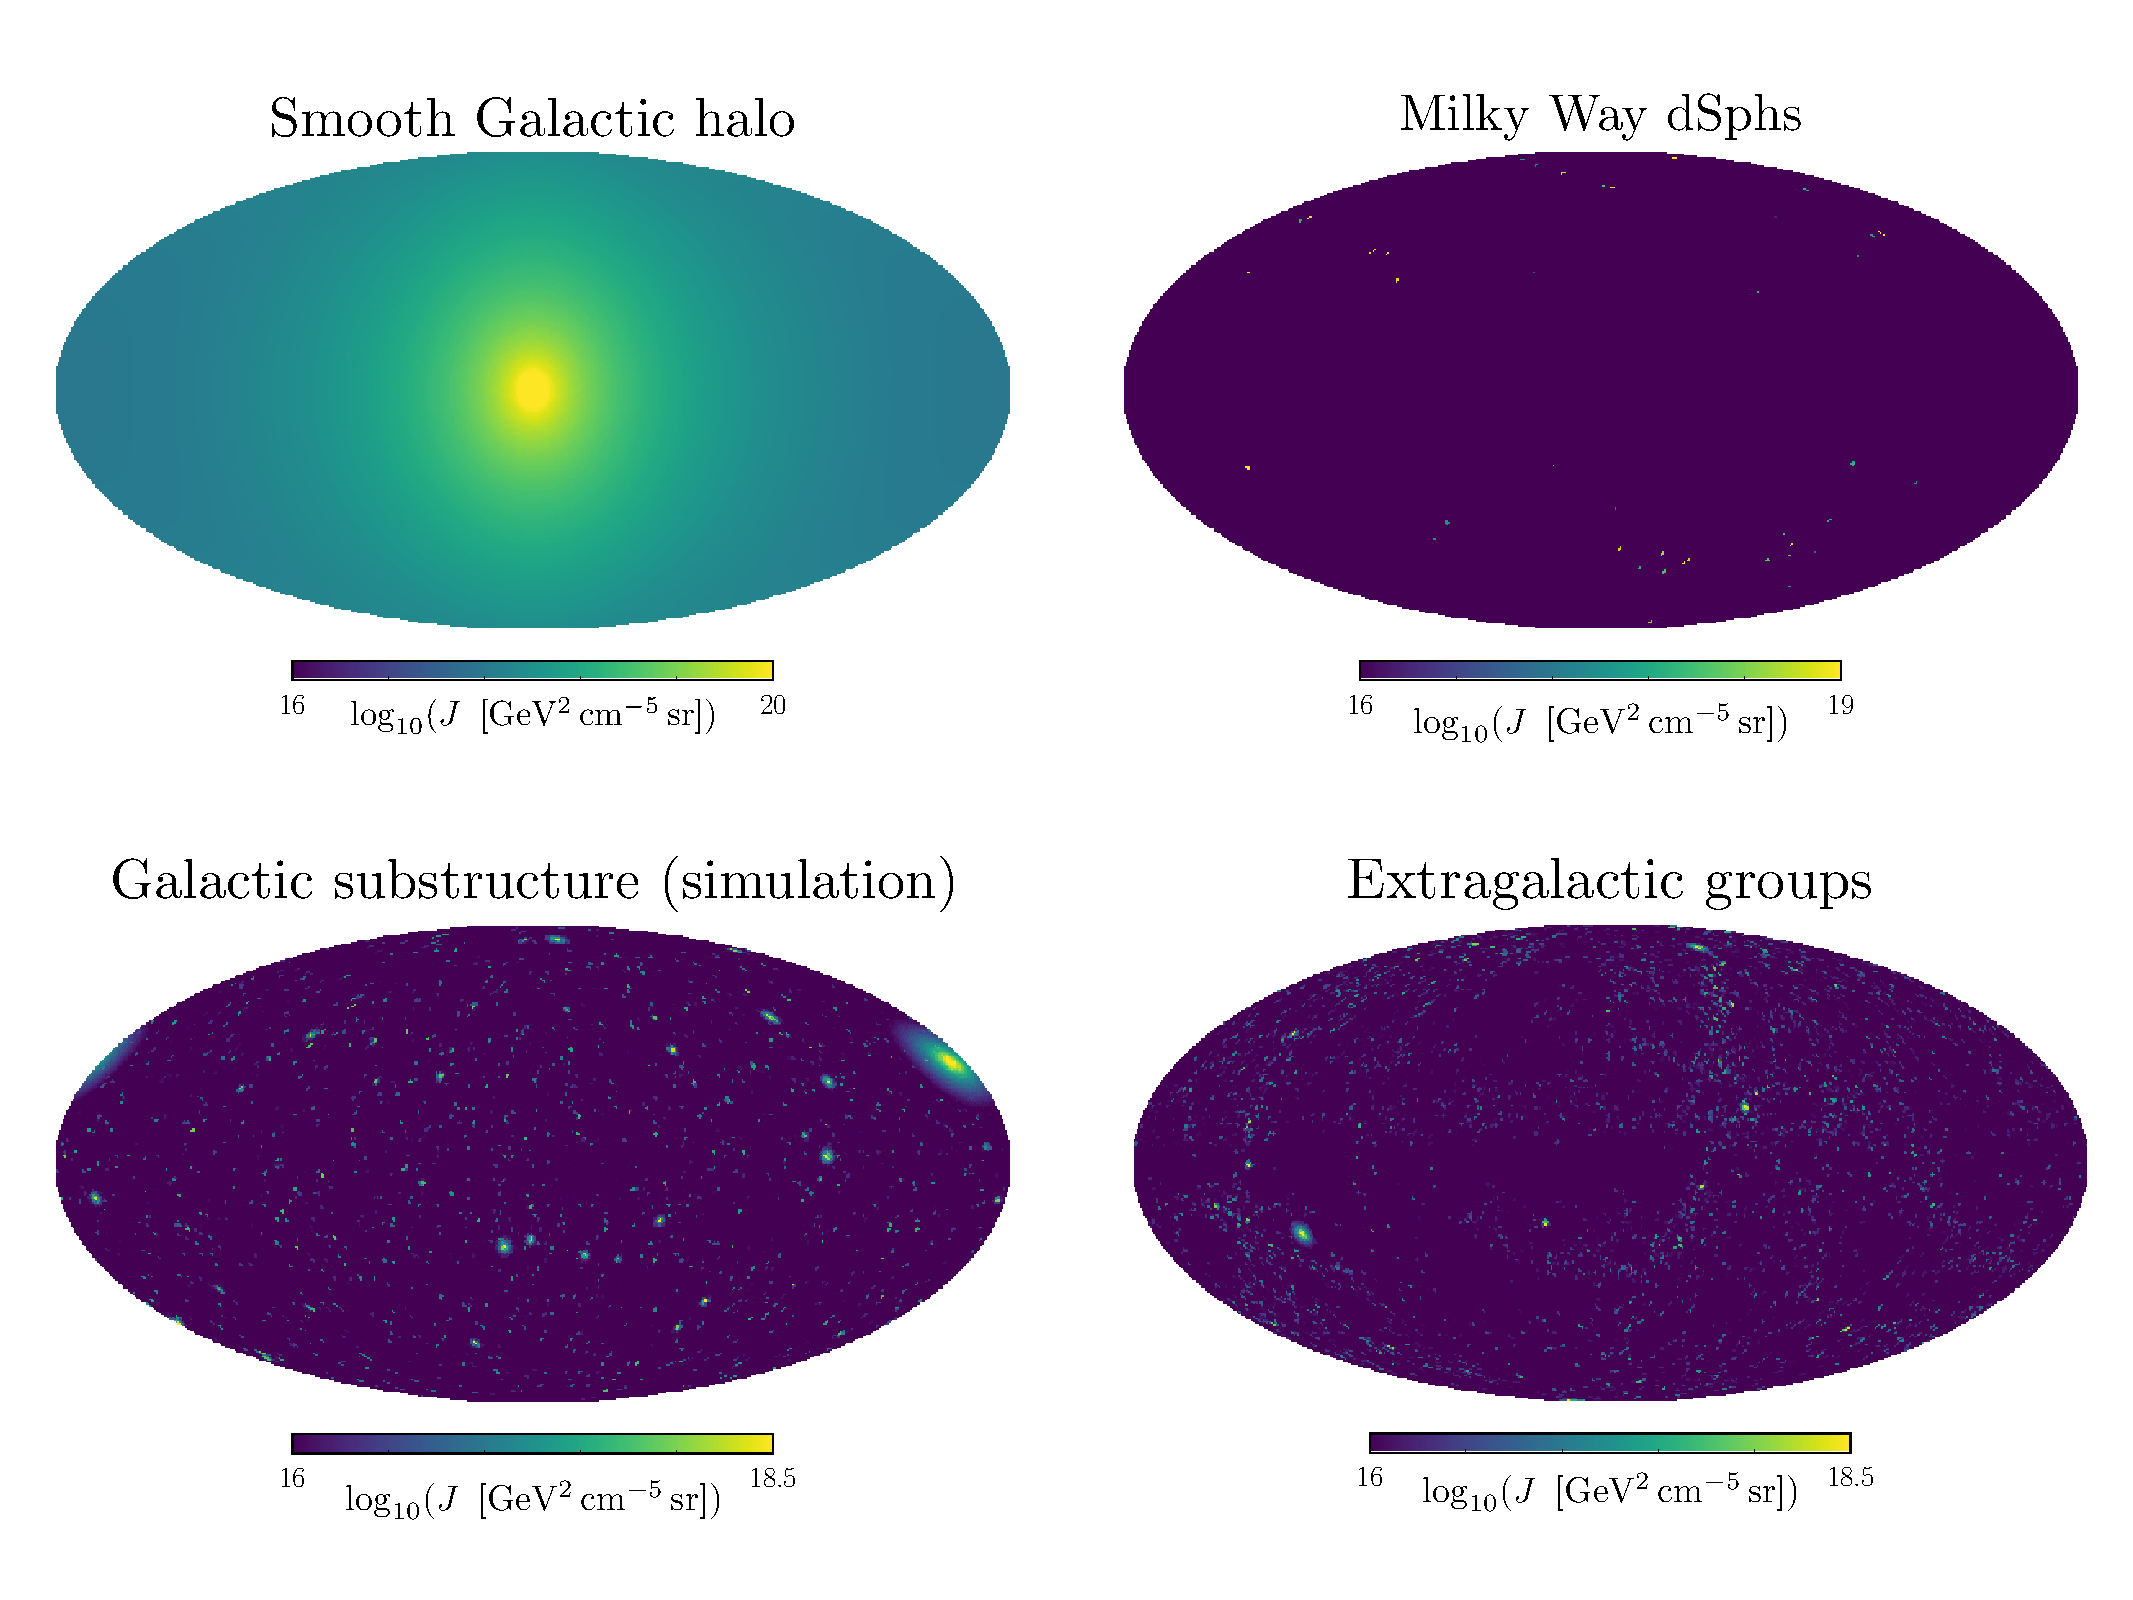
\includegraphics[width=1.0\textwidth]{ch-intro/jfactors.pdf}
\caption{Maps of annihilation $J$-factors for some commonly considered gamma-ray search targets. \textbf{(Top left)} The smooth Galactic halo, assuming a canonical NFW dark matter profile $\rho_\text{NFW}(r)=\frac{\rho_{s}}{r/r_{s}\,(1+r/r_{s})^{2}}$, where $r_s=17$ kpc is the Milky Way scale radius and $\rho_s$ is the normalization chosen to reproduce the local DM density $\rho_\text{NFW}(r_\odot) = 0.4$ GeV$\,$cm$^{-3}$~\cite{2015ApJ...814...13M,Sivertsson:2017rkp} at the Solar radius $r_\odot = 8$~kpc~\cite{Read:2014qva}. \textbf{(Top right)} Milky Way dwarf spheroidal galaxies (dSphs) as considered in Ref.~\cite{Fermi-LAT:2016uux}. Following that study, the dSphs are assumed to be point-like sources since the properties of the corresponding DM halos are not currently well constrained. \textbf{(Bottom left)} A simulated realization of $J$-factors for Galactic substructure (subhalos) following the prescription in~\cite{Hutten:2016jko}. Subhalos are spatially distributed according to the results of the Aquarius simulation~\cite{Springel:2008cc} and a halo mass distribution of $dN/dm\propto m^{-1.9}$ is assumed. The concentration-mass parameterization from Ref.~\cite{Sanchez-Conde:2013yxa} is used and DM in the subhalos is assumed to be NFW-distributed. The number of subhalos is calibrated to give 300 objects between $10^8$--$10^{10}$\,M$_\odot$. The bright source in the top right corner of the map would likely show up as a resolved unassociated source in \emph{Fermi} point source catalogs such as 3FGL~\cite{Bertoni:2015mla}. \textbf{(Bottom right)} $J$-factors of extragalactic groups derived using properties compiled in the group catalogs of Refs.~\cite{Tully:2015opa} and~\cite{2017ApJ...843...16K} and the prescription presented in Chs.~\ref{ch:groups_sim} and \ref{ch:groups_data}.}  
\label{fig:sources}
\end{figure}


\subsection{Template Methods for Gamma-Ray Searches}
\label{subsec:statmethods}

Data from gamma-ray detectors such as \emph{Fermi}-LAT is typically a series of sky maps, representing the number of photons binned spatially as well as in energy. Figure~\ref{fig:data} shows a subset of a typical \emph{Fermi}-LAT dataset. In analyzing such data within the context of dark matter indirect detection, the challenge lies in have contributions from large-scale structures such as the smooth Galactic halo as well as point/extended sources like dwarf galaxies, from various astrophysical backgrounds. The most common technique for characterizing the various potential sources that contribute to gamma-ray data is Poissonian template fitting, which is briefly described here; a detailed description will be given in Ch.~\ref{ch:groups_sim}. 

\begin{figure}[htbp] 
\centering
 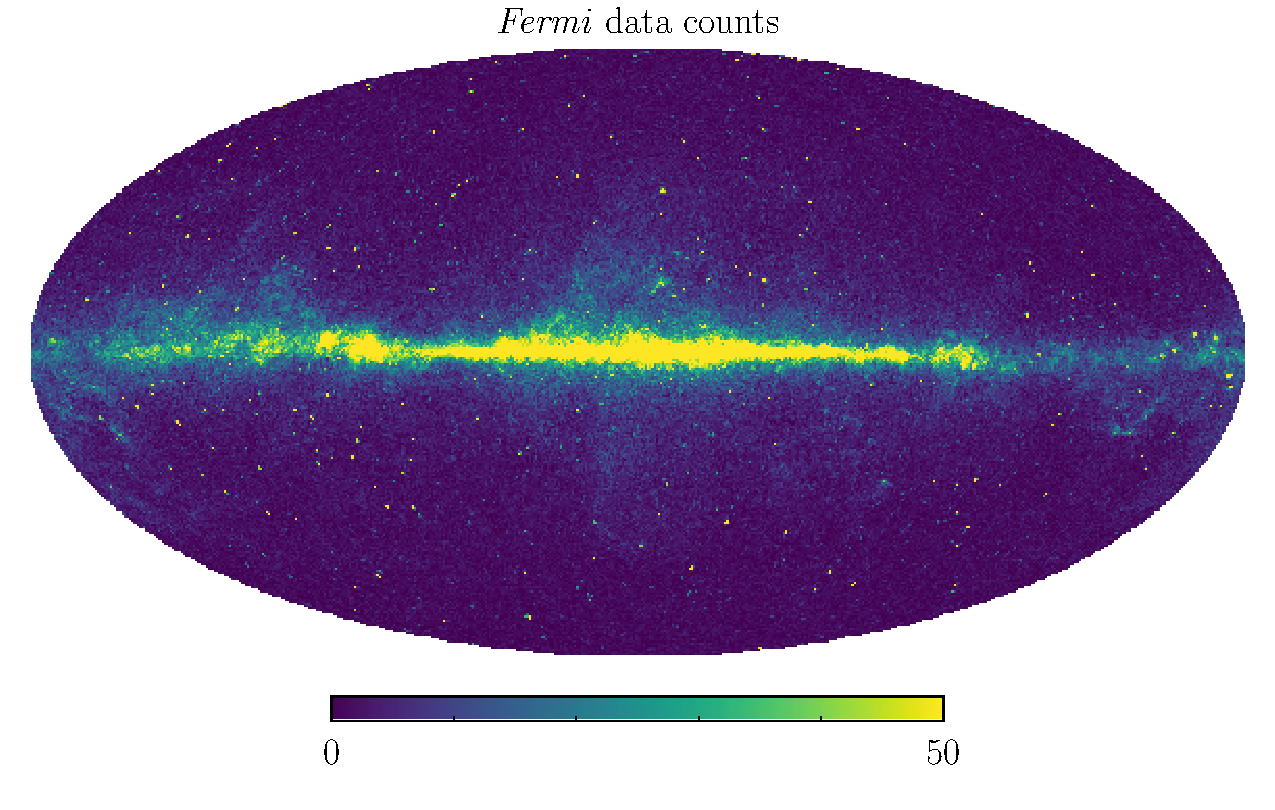
\includegraphics[width=0.8\textwidth]{ch-intro/data.pdf}
\caption{A subset of the photons collected by \emph{Fermi}-LAT between August 4, 2008 and July 7, 2016, in the energy range 2--20 GeV. The visualization is of the top quartile of the UltracleanVeto event class (PSF3) as ranked by angular resolution, with the recommended quality cuts applied (see Ch.~\ref{ch:groups_sim} for further details).}  
\label{fig:data}
\end{figure}

A template is a spatial map which traces the modeled contribution of a particular source or class of sources to the data, \emph{e.g.} the expected emission from the diffuse Galactic foreground or resolved astrophysical point sources. Figure~\ref{fig:templates} shows some templates commonly used in \emph{Fermi} gamma-ray analyses (see caption for descriptions). Templates for DM emission can be constructed as described in Secs.~\ref{subsec:tools} and \ref{subsec:dmsources}. 

Within a single energy bin, if we denote the value of a given template $i$ in pixel $p$ by $T_i^p$, then the total expected counts in pixel $p$ is given by 
\begin{equation}
\mu^p(\boldsymbol \theta) = \sum_i A_i\,T_i^p,
\end{equation}
where $\boldsymbol \theta$ represents the signal and background model parameters ${A_i}$, which in this case are the normalizations of the corresponding templates. The observed data in pixel $p$ should therefore be a Poisson realization of the sum of modeled components. It follows that the likelihood function for the parameters $\boldsymbol \theta$ given the data $d$ is a product over all pixels in the region-of-interest of the Poisson probabilities associated with observing $n^{p}$ counts in each pixel $p$:
\begin{equation}
\mathcal{L}(d | {\boldsymbol \theta}) = \prod_p \frac{\mu^{p}({\boldsymbol \theta})^{n^{p}} e^{-\mu^{p}({\boldsymbol \theta})}}{n^{p}!}\,.
\label{eq:pi}
\end{equation}
With the likelihood in hand, we can quantify the contribution of various components using conventional inference methods, \emph{e.g.} obtaining posterior distributions within a Bayesian framework or building up a likelihood surfaces using frequentist profile likelihood techniques. The latter is more commonly used in DM searches---typically, we are more interested in the parameters associated with the DM model (\emph{e.g.} its particle mass $m_\chi$ and annihilation cross section $\langle\sigma v\rangle$, which are in 1-to-1 correspondence with the normalization of the DM template) than those corresponding to the astrophysical backgrounds. A likelihood surface $\mathcal{L}(d|\mathcal M, \{m_\chi, \langle\sigma v\rangle\})$ for the signal parameters corresponding to a given DM model $\mathcal M$ can be obtained by maximizing the likelihood with respect to the background parameters at each signal parameter point. This can be generalized to the cases of analyzing several energy bins and/or stacking multiple sources (\emph{e.g.} several extragalactic halos), where the total likelihood would be given by the product of the individual likelihoods.

For inferring dark matter properties, a log-likelihood difference test statistic (TS) can be defined for a given mass $m_\chi$ as
\begin{equation}\begin{aligned}
{\rm TS}(\mathcal{M}, \{ \langle\sigma v\rangle, m_\chi\}) \equiv 2 &\left[ \log \mathcal{L}(d | \mathcal{M}, \{\langle\sigma v\rangle, m_\chi \}) \right.\\
&\left.- \log \mathcal{L}(d | \mathcal{M}, \{{\langle\sigma v\rangle=0}, m_\chi \}) \right]\,,
\label{eq:TSdef_darksky}
\end{aligned}\end{equation}
% where $\widehat{\langle\sigma v\rangle}$ is the cross section corresponding to the maximum value of the likelihood for a given DM model $\mathcal M$ and mass $m_\chi$. We define the TS with respect to this maximum value in order to set a conservative limit in the presence of background mismodeling or a potential signal. 
where $\langle\sigma v\rangle=0$ corresponds to the null signal hypothesis. Wilks' theorem guarantees that in the asymptotic limit of a large sample size, the TS is $\chi^2$-distributed, allowing us to discover (if we're lucky) or exclude a DM signal in the data to a desired statistical significance in accordance with $\chi^2$ statistics. A TS value of $-2.71$, for example, corresponds to exclusion at a confidence level of 95\%. Modified versions of this statistical procedure will be used in Chs.~\ref{ch:groups_sim} and \ref{ch:groups_data} to look for DM annihilation in extragalactic galaxies and clusters.

A fundamental limitation of Poissonian template fitting is that while resolved point sources can be either modeled with templates or masked, this is not possible for dim, sub-threshold point sources that cannot be detected individually. Depending on their spatial distribution, emission from these unresolved point sources is typically absorbed by other extended templates, \emph{e.g.} isotropic (in the case of extragalactic sources) or Galactic dark matter (in the case of an approximately spherically symmetric population of unresolved sources in the Galactic center). Chapter~\ref{ch:nptfit} will be dedicated to extending traditional Poissonian template fitting methods to statistically account for the presence of unresolved point sources in the data.

\begin{figure}[htbp] 
\centering
 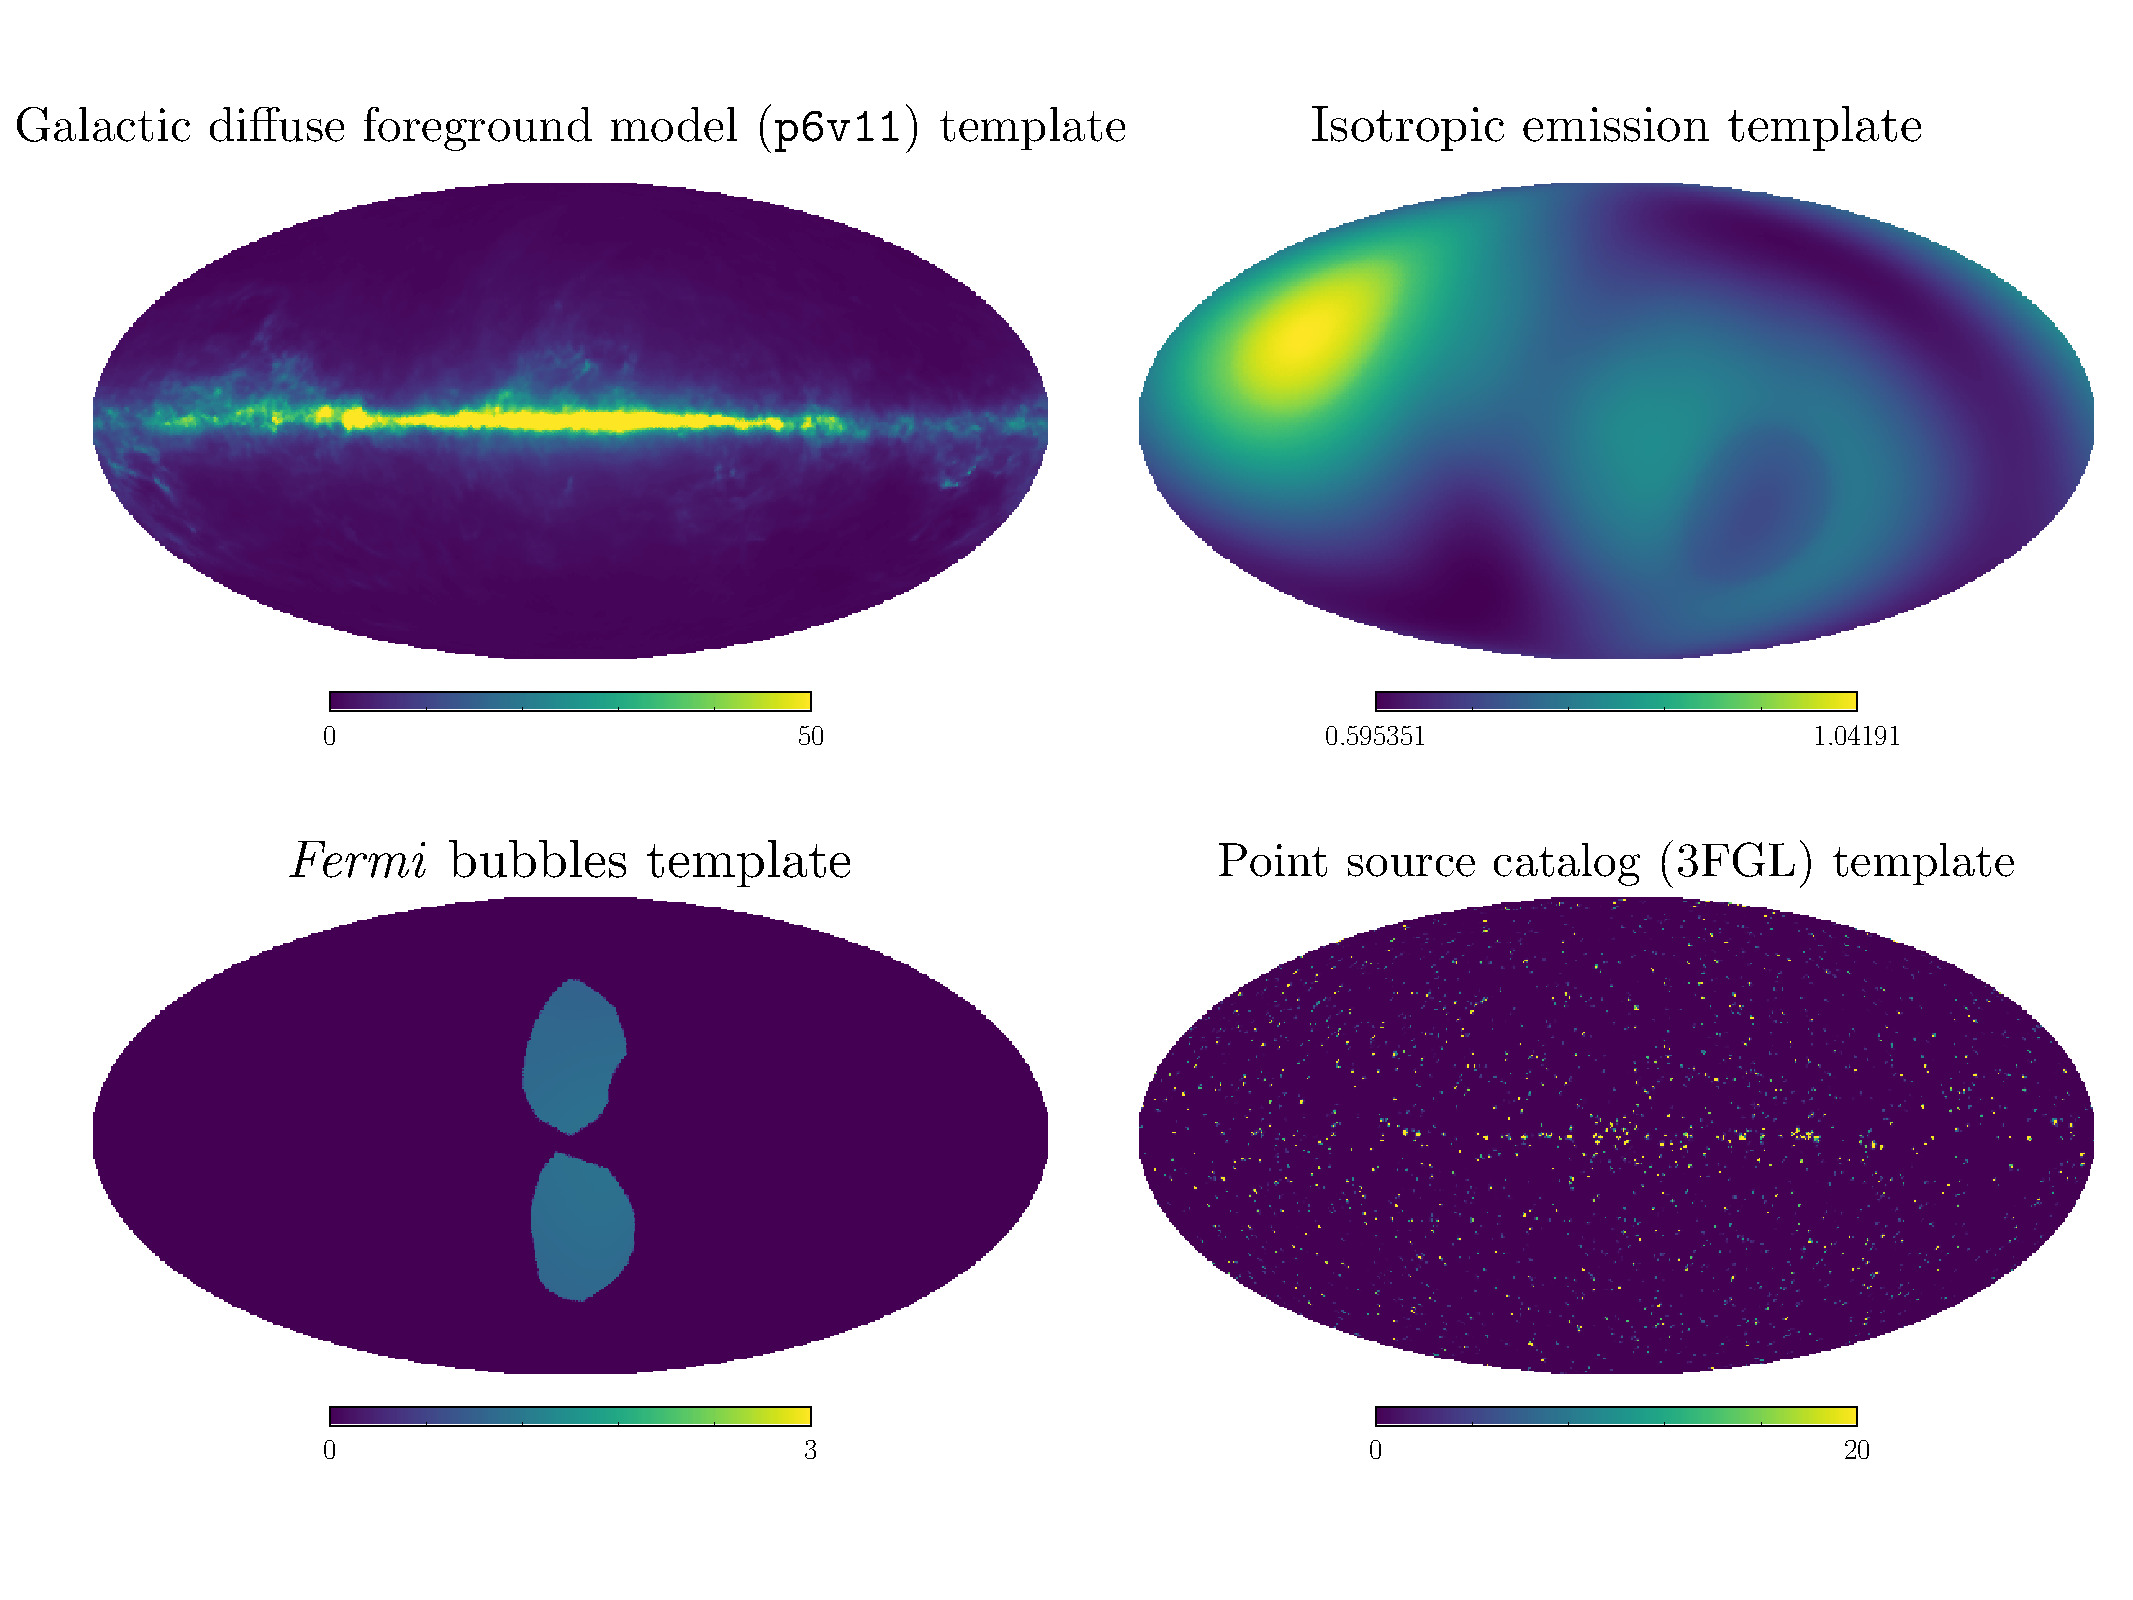
\includegraphics[width=1.0\textwidth]{ch-intro/templates.pdf}
\caption{Representative templates commonly considered in \emph{Fermi}-LAT gamma-ray analyses. The normalizations of the templates correspond to the best-fit values to the data shown in Fig.~\ref{fig:data}. \textbf{(Top left)} Template for the Galactic diffuse foreground emission, as modeled by the  {\it Fermi} \texttt{p6v11} model. \textbf{(Top right)} Isotropic template, intended to account for emission from unresolved extragalactic point sources. This template is not perfectly uniform due to the non-uniform exposure of the LAT instrument. \textbf{(Bottom left)} Template for the \emph{Fermi} bubbles, two lobe-like structures likely of astrophysical origin~\cite{Su:2010qj,Fermi-LAT:2014sfa}. \textbf{(Bottom right)} Template for resolved point sources as compiled in the \emph{Fermi} 3FGL catalog~\cite{Acero:2015hja}.}  
\label{fig:templates}
\end{figure}

\section{Thesis Organization}
\label{sec:summary}

The rest of this thesis is organized as follows. Chapter~\ref{ch:nptfit} describes the implementation of a novel statistical method, first introduced in Ref.~\cite{Lee:2015fea}, which leverages the ``clumpiness'' of photons associated with populations of unresolved point sources (PSs) in astronomical datasets to derive their contribution and properties. In Ch.~\ref{ch:igrb}, this method is applied to the gamma-ray sky at higher latitudes as seen by \emph{Fermi} to characterize the contribution of PSs to the extragalactic gamma-ray sky over three order of magnitude in energy, from 2 to 2000 GeV. Chapter~\ref{ch:groups_sim} asks the question: ``what is the best way to look for annihilating dark matter in extragalactic sources?'' and attempts to answer it by constructing a pipeline to robustly map out the distribution of dark matter in the local neighborhood using galaxy group catalogs. Uncertainties involved in inferring various dark matter parameters are discussed in detail. In Ch.~\ref{ch:groups_data}, this framework is applied to \emph{Fermi} data and existing group catalogs to search for annihilating dark matter in local galaxies and clusters, and stringent bounds are obtained in the absence of a signal. 

\sectionline

% \begin{itemize}
% \item History of dark matter

% \item Particle dark matter
% \item The case for WIMPs 
% \item Dark matter searches
% \end{itemize}